\chapter{Tagging--Systeme}
\label{tagging}

Das folgende Kapitel beschäftigt sich mit Tagging--Systemen. Dabei werden die Grundlagen, das Datenmodell und die Arten von Tagging--Systemen erläutert sowie das System von Spreadshirt, das in dieser Arbeit verwendet wurde, genauer erklärt. Dies umfasst die spezifischen Eigenschaften dieses Systems, die Diskussion der Datenqualität sowie das Mengengerüst der vorhandenen Daten.

\section{Grundlagen}
\label{tagging_basics}

\emph{Tags} sind eine Form von Metadaten, also ``Daten über Daten''. Sie erfüllen die Funktion der \emph{Beschreibung} von Dokumenten und werden im Allgemeinen von Benutzern angelegt. Dies steht im Gegensatz zu professionell kuratierten Metadaten wie beispielsweise Bibliothekskatalogen \cite{ma2004}.

Im Allgemeinen sind Tags kurze Schlagworte, die von dem Benutzer, der sie vergibt, frei gewählt werden können. Jedes Dokument kann mit beliebig vielen Tags versehen werden. Dies steht im Gegensatz zu einer festen, vorgegebenen Klassifikation mittels Kategoriebäumen, wie sie beispielsweise in E--Commerce--Systemen üblich sind, um Artikel zu ordnen. In solchen Kategoriebäumen kann ein Dokument üblicherweise nur in einer begrenzten Anzahl von Kategorien, meistens nur in einer, eingeordnet werden.

Die Menge der Tags eines Systems ist nicht hierarchisch geordnet und es bestehen keine explizit formulierten Beziehungen zwischen einzelnen Tags. Somit ergibt sich eine lose Kategorisierung der Dokumente, die, im Gegensatz zu formalen Taxonomien und Ontologien, ständig von den Benutzern erweitert und verändert wird \cite{sc2005}. \textcite{je2004} beschäftigt sich tiefer gehend mit dem Unterschied zwischen starrer Klassifikation und loser Kategorisierung.

Aus dieser Eigenschaft ergeben sich bestimmte Schwächen und Stärken von Tagging--Systemen, die von \textcite{ma2004} definiert wurden. Demnach liegen die Schwächen in der Mehrdeutigkeit von Tags und der mangelnden Kontrolle von Synonymen. Mehrdeutigkeit bezeichnet den Umstand, dass gleiche Tags zur Beschreibung von sehr unterschiedlichen Dokumenten genutzt werden können, da keine Systematik vorgegeben ist. Die mangelnde Kontrolle von Synonymen führt dazu, dass verschiedene Tags verwendet werden, um den gleichen Sachverhalt zu beschreiben.

Zu den von \textcite{ma2004} formulierten Stärken gehören die starke Ausrichtung von Tags an den Gedankengängen der Benutzer und dem einfacheren Durchstöbern von Dokumenten. Da die Tags von den Benutzern eines Systems formuliert werden, spiegeln sie deren Vokabular und deren Gedankengänge wieder. Werden Tags statt zum Finden von konkreten Dokumenten zum Durchstöbern genutzt, bieten sie größere Möglichkeiten, interessante Inhalte zu finden, als in einer starren Kategorisierung.

Tagging--Systeme enthalten also implizites Wissen, dass durch Data Mining extrahiert und genutzt werden kann. Im Rahmen dieser Arbeit wurden Tagging--Systeme als Ausgangspunkt für die Link Discovery mittels Kookkurrenz genutzt genutzt (siehe \cref{co-occurence,ld_tags}).

\subsection{Datenmodell von Tagging--Systemen}
\label{tagging_data}

Ein Tagging--System ist allgemein durch ein Tripel \(S=(D, T, U)\) von Mengen, sowie durch die Relation \(R = D \times U \times T\) definiert. 

\(D\) repräsentiert eine Menge von Dokumenten. Ein Dokument \(d\) kann ein beliebiger Datensatz sein, beispielsweise ein Design, Artikel oder Produkt. Die Menge \(U\) stellt alle Benutzer des Systems dar. Ein Benutzer \(u\) ist eine Entität mit beliebigen weiteren Attributen, die jedoch im Kontext des Tagging--Systems nicht weiter betrachtet werden. \(T\) repräsentiert die Menge der Tags. Ein Tag \(t\) ist eine Entität, die als benötigtes Attribut eine Zeichenkette besitzt, die zur Beschreibung von Dokumenten genutzt werden kann. \(T\) bildet das \emph{Vokabular} des Tagging--Systems.

Die Relation \(R\) beschreibt den Vorgang des \emph{Taggings}. Ein Benutzer \(u\) des Systems vergibt dabei einen Tag \(t\) an ein Dokument \(d\), um den Inhalt von \(d\) mit der Zeichenkette von \(t\) zu beschreiben. \(R\) enthält demnach Tripel der Form \((d,t,u)\).

\begin{figure}
\centering
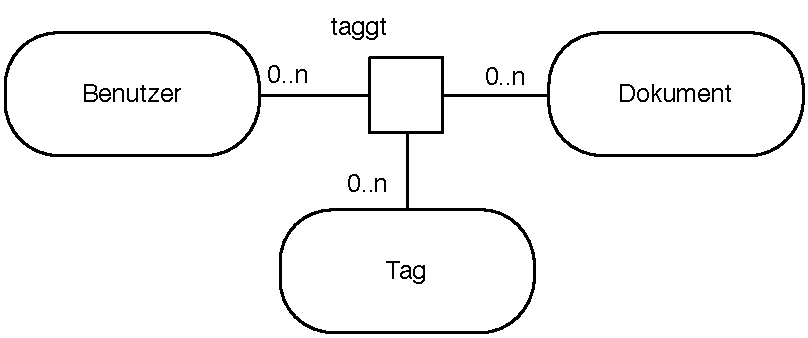
\includegraphics[width=0.75\textwidth]{tag_system}
\caption{FMC--Entity--Relationship--Diagramm eines Tagging--Systems}
\label{fig:tagging_erd}
\end{figure}

Das beschriebene Tagging--System lässt sich somit in ein Datenmodell mit den Entitäten \emph{Benutzer}, \emph{Dokument}, \emph{Tag} und  der ternären Beziehung \emph{Tagging} überführen. Dieses Modell ist in \cref{fig:tagging_erd} als Entity--Relationship--Diagramm dargestellt. Alle genannten Entitäten können weitere Attribute besitzen, die von der Anwendungsdomäne des konkret betrachteten Tagging--Systems abhängen.

\subsection{Arten von Tagging--Systemen}
\label{tagging_types}

Abhängig vom gewünschten Einsatzzweck des Tagging--Systems kann der Betreiber bestimmte Aspekte des Systems beschränken. Außerdem können die Benutzer einen vorherrschenden Umgang mit dem System entwickeln. Aus diesen Faktoren ergeben sich verschiedene Arten und Nutzungsmuster von Tagging-Systemen. Hauptsächlich kann zwischen offenen Tagging--Systemen, den so genannten \emph{Folksonomies} und den teilweise geschlossenen Tagging--Systemen unterschieden werden.

\subsubsection{Folksonomies}

Eine Folksonomy beschreibt ein weitestgehend offenes Tagging--System \cite{ma2004}. Bei dieser Art von System kann grundsätzlich jeder Benutzer jeden Tag an jedes Dokument vergeben. Außerdem stammen die Dokumente selbst meist ebenfalls von den Benutzern. Beispiele für Folksonomies sind der Bookmarking--Dienst \emph{Delicious} \cite{deli} und die Foto-Plattform \emph{Flickr} \cite{flickr}.

Der Begriff \emph{Folksonomy} steht dabei im Gegensatz zur \emph{Taxonomie} und beschreibt den Umstand, dass die Kategorisierung und Ordnung von Inhalten vom \emph{folk}, also den Benutzern selbst vorgenommen werden \cite{vt2007}.

\subsubsection{Teilweise geschlossene Tagging--Systeme}

In teilweise geschlossenen Tagging--Systemen beschränkt der Betreiber des Systems bestimmte Aspekte. Dies können die Benutzer, die Tags vergeben dürfen, die Dokumente oder auch das Vokabular sein.

Eine häufige Form der Einschränkung, der auch das in dieser Arbeit verwendete System unterliegt (siehe \cref{tag_sprd}), ist die Einschränkung der Benutzer die ein Dokument taggen können. Oftmals ist dies nur den Autoren des Dokumentes selbst oder Benutzern mit besonderen Rechten, beispielsweise Moderatoren oder Angestellten des Betreibers, erlaubt.

In den meisten Tagging--Systemen stammen die Dokumente ebenfalls von den Benutzern des Systems, beispielsweise Artikel, Fotos oder Musikstücke. Jedoch kann die Erstellung der Dokumente eingeschränkt werden, wenn dies in der Anwendungsdomäne sinnvoll ist. Beispiele hierfür sind Produkte in Online--Shops. Diese werden nicht von den Benutzern erstellt, jedoch kann die Vergabe von Tags an diese einen Mehrwert liefern.

Die Einschränkung des Vokabulars kann vorgenommen werden, um Rechtschreibfehler und Fehleingaben der Tags zu vermeiden. Sie bringt jedoch den Nachteil mit sich, dass die Tags dann unter Umständen nicht mehr das Vokabular der Benutzer widerspiegeln und somit Inhalte für diese schwerer auffindbar sind.

\section{Tagging--System von Spreadshirt}

Nachdem im vorherigen Abschnitt die Grundlagen von Tagging--Systemen diskutiert wurden, beschäftigt sich dieser Abschnitt mit dem konkreten Tagging--Systems der Website \emph{Spreadshirt}, welches in dieser Arbeit für den initialen Schritt der Link Discovery genutzt wurde (siehe \cref{ld_tags}).

\subsection{Spreadshirt}
\label{spreadshirt}

Die vorliegende Masterarbeit wurde im Kontext der sprd.net AG (Spreadshirt) \cite{sprd2013} erstellt. Spreadshirt ist eine E--Commerce--Plattform, die es seinen Benutzern erlaubt, personalisierte Textilien und andere Artikel zu gestalten, zu kaufen und zum Verkauf anzubieten. Spreadshirt übernimmt die Produktion und den Versand der Produkte. Ein Produkt bezeichnet hierbei einen Produkttyp, beispielsweise ein T--Shirt, der mit einem oder mehreren Designs bedruckt wurde.

Das Erstellen von Designs und die Konfiguration eines Produktes, also das Positionieren von Designs auf Produkttypen, wird vollständig vom Benutzer durchgeführt. Es agieren grundsätzlich zwei Arten von Benutzern mit der Spreadshirt--Plattform: \emph{Kunden} und \emph{Partner}.

Als Kunden werden Benutzer bezeichnet, die Produkte bestellen. Diese Produkte können entweder von ihnen selbst oder von einem Partner erstellt worden sein. 

Partner sind Benutzer, die Designs oder Produkte erstellen und diese zum Verkauf anbieten. Zu diesem Zweck kann der Partner einen eigenen Shop auf der Spreadshirt--Plattform eröffnen. Kunden können in diesem Shop Produkte bestellen und der Partner erhält einen Anteil des Verkaufspreises, während Spreadshirt die Produktion und den Versand an den Kunden übernimmt.

Neben den von Kunden für sich selbst erstellten Produkten und den Partner--Shops existiert mit dem Spreadshirt--Marktplatz ein weiterer Vertriebskanal. Auf dem Marktplatz können Partner nach ihrer Zustimmung ihre Designs vertreiben. Kunden können nach Motiven suchen, die ihrem Geschmack entsprechen und diese bestellen, mit anderen Motiven kombinieren oder mit Texten versehen. Ein Produkt, das entweder in einem Partner--Shop oder auf dem Marktplatz positioniert und mit einem Preis versehen wurde, wird Artikel genannt.

\begin{figure}[t]
\centering
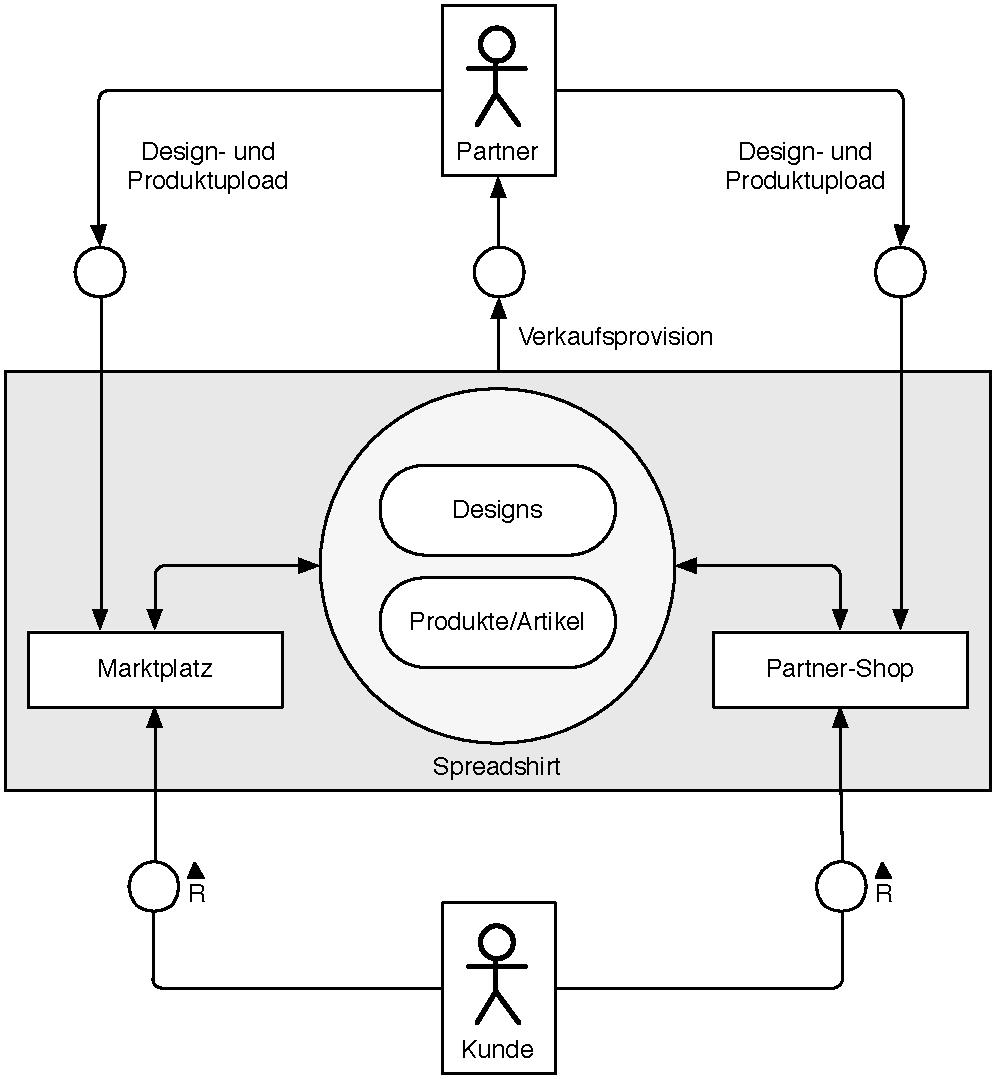
\includegraphics[width=0.65\textwidth]{how_spreadshirt_works}
\caption{FMC--Blockdiagramm der Spreadshirt--Bereiche und Benutzer}
\label{fig:howspreadshirtworks}
\end{figure}

Die grundsätzliche Funktionsweise der Spreadshirt--Plattform ist in \cref{fig:howspreadshirtworks} als FMC--Blockdiagramm dargestellt.

Das Suchergebnis für Suchen auf dem Marktplatz hängt maßgeblich von den Metadaten ab, die der Partner für seine Designs vergeben hat. Dazu gehören Tags, aber auch Titel und Beschreibung des Designs oder Produktes. In dieser Arbeit wird ausschließlich das Tagging--System betrachtet.

\label{platforms}
Spreadshirt betreibt aus historischen Gründen zwei Plattformen, deren Datenbestände größtenteils voneinander getrennt sind. Jeweils eine Plattform ist für den nordamerikanischen und den europäischen Markt zuständig. Im Kontext dieser Arbeit wird die europäische Plattform als Ausgangsbasis für alle Betrachtungen gewählt. Der Datenbestand dieser Plattform besteht aus circa 2 Millionen Tags, 6 Millionen Designs, 14 Millionen Produkten, 6 Millionen registrierten Nutzern und \num{750000} eröffneten Partner--Shops.

\subsection{Eigenschaften des Tagging--Systems}
\label{tag_sprd}

Im Fall von Spreadshirt ist die Vergabe von Tags auf die Menge der Partner \(P \subseteq U\) begrenzt (siehe auch \cref{spreadshirt}). Es handelt sich demnach um ein in \cref{tagging_types} beschriebenes teilweise geschlossenes Tagging--System.

Die Dokumente, die von den Partnern getaggt werden können, sind auf die Designs und Artikel beschränkt, die der Partner selbst angelegt hat. Eine Beschreibung kann also ausschließlich durch den Autor des Inhaltes erfolgen. Deshalb fehlt im Vergleich zu anderen Tagging--Systemen auch die Information, welcher Benutzer den Tag vergeben hat, da diese implizit durch den Autor des Dokumentes gegeben ist.

Des Weiteren besitzen Tags in der Spreadshirt--Datenbank ein Attribut \emph{Sprache} aus der Menge \(L\). Die Sprache spielt bei der Eingabe und Anzeige der Tags zu Dokumenten eine Rolle. Je nach eingestellter Sprache auf der Website erstellt und sieht der Benutzer nur Tags, die mit dieser Sprache markiert sind.

Das Vokabular der Tags ist nicht eingeschränkt. Dies bringt zwangsläufig Probleme der Datenqualität mit sich, welche im folgenden Abschnitt erläutert werden.

\subsection{Datenqualität des Tagging--Systems}
\label{quality}

Die Qualität von Daten wird im Allgemeinen unter mehreren Gesichtspunkten beurteilt. Dazu gehören unter anderem \emph{Korrektheit}, \emph{Vollständigkeit}, und \emph{Redundanzfreiheit} \cite[S. 84 f.]{hkp2012}. Nachfolgend werden die bei Spreadshirt vorhandenen Tagging--Daten nach diesen Kriterien betrachtet und die Quellen eventueller Fehler \cite[S. 43 f.]{jo2003} diskutiert.

\subsubsection{Korrektheit}

Die Korrektheit der Tagging--Daten kann an vielen Punkten angezweifelt werden. Das hervorstechende Problem hierbei ist das Auftreten von Spam. Viele Partner versehen ihre Artikel und Designs mit Tags, die nicht den Inhalt beschreiben. Partner versehen ihre Designs und Artikel mit falschen Tags, damit diese bei populären Suchbegriffen gefunden werden.

Ein weiterer Defekt ist die Inkorrektheit des Attributes \emph{Sprache} der Tags. Die Sprache wird aus der Domain abgeleitet, die der Benutzer, der den Tag eingegeben hat, besucht hat. Viele Partner geben jedoch ihre Tags in mehreren Sprachen ein, um ihre Inhalte besser auffindbar zu machen. Dies führt in der Konsequenz dazu, dass das Attribut Sprache in einem nicht unwesentlichen Teil der Tags als falsch angesehen werden kann.

Die Quelle beider Fehler ist also die bewusste Falscheingabe von Informationen, um einen persönlichen Vorteil zu erlangen, da die Partner versuchen, ihre Produkte möglichst zu vielen Sucheingaben in den Ergebnissen auftauchen zu lassen.
                                                                                                                                                                                                                                                                                                                                                                                                              
\subsubsection{Vollständigkeit}

Wie bereits in \cref{tag_sprd} beschrieben, fehlen in den Daten des Spreadshirt--Systems der Zeitpunkt und der Benutzer eines Taggings. Dies führt in der Konsequenz dazu, dass Spam schwerer erkannt werden kann. Zwar ist bekannt, wann ein Tag das erste Mal verwendet wurde, alle weiteren Verwendungen des Tags haben jedoch keinen Zeitstempel. Der Benutzer, der den Tag angelegt und verwendet hat, kann nur daraus abgeleitet werden, wer den getaggten Artikel angelegt hat.

Die Unvollständigkeit der Daten rührt in erster Linie daher, dass zum Zeitpunkt der Implementierung des Tagging--Systems noch nicht bedacht wurde, dass die fehlenden Attribute später nützlich sein können.

\subsubsection{Redundanzfreiheit}

Bedingt durch die Form der Dateneingabe besteht für das Vokabular des Tag--Systems ein großes Potential für redundante Daten. Da eingegebene Tags durch einen Separator getrennt eingegeben werden müssen, besteht hier Potential zur Fehleingabe. Wird der falsche Separator verwendet, werden die eigentlich getrennten Tags als eine einzige Entität abgespeichert.

Technisch kann jeder Tag genau ein Mal in der Datenbank vorkommen. Jedoch führen Tipp-- und Rechtschreibfehler, unterschiedliche Groß- und Kleinschreibung, verschiedene Arten zusammengesetzte Wörter zu schreiben, Leerräume vor, nach und zwischen Wörtern eines Tags und Tippfehler dazu, dass das gleiche Wort mehrfach in der Datenbank gespeichert wurde.

Außerdem führten in der Vergangenheit Systemfehler und Implementierungsfehler dazu, dass falsche, nicht druckbare Zeichen in den Tags enthalten waren. Nach Beseitigung der Fehler blieben die fehlerhaften Tags bestehen, so dass bei einer erneuten Eingabe des gleichen Wortes ein neuer Tag in der Datenbank angelegt wurde.

\subsection{Mengengerüst des Tagging--Systems}

Zum Zeitpunkt der Bearbeitung dieser Arbeit befanden sich im Datenbestand der europäischen Spreadshirt--Plattform:

\begin{itemize}
    \item \num{2072079} Tags in \num{15} verschiedenen Sprachen
    \item \num{6433410} Benutzer
    \item \num{26147860} Dokumente (\num{16494430} Artikel und \num{9653430} Designs)
    \item \num{71938905} Taggings
\end{itemize}

Diese Datenmengen stellen besondere Anforderungen an die Verarbeitung. Wie diese umgesetzt wurden, wird in \cref{system} diskutiert.

\section{Zusammenfassung}

Dieses Kapitel befasste sich mit Tagging--Systemen. Dazu wurden die Grundlagen und Begriffe genannt, die Vor-- und Nachteile von Tagging--System erläutert, das Datenmodell formalisiert und die grundsätzlichen Arten Folksonomy und teilweise geschlossenes Tagging--System unterschieden.

Außerdem wurde das im weiteren Verlauf dieser Arbeit verwendete Tagging--System von Spreadshirt \cite{sprd2013} näher betrachtet. Dazu wurden die speziellen Eigenschaften dieses Systems, die Datenqualität und die Menge der vorhandenen Daten beschrieben.

Das nachfolgende Kapitel beschäftigt sich mit dem zur Link Discovery angewandten Framework.